\section{Blue Live}\label{blueLive}

Blue Live

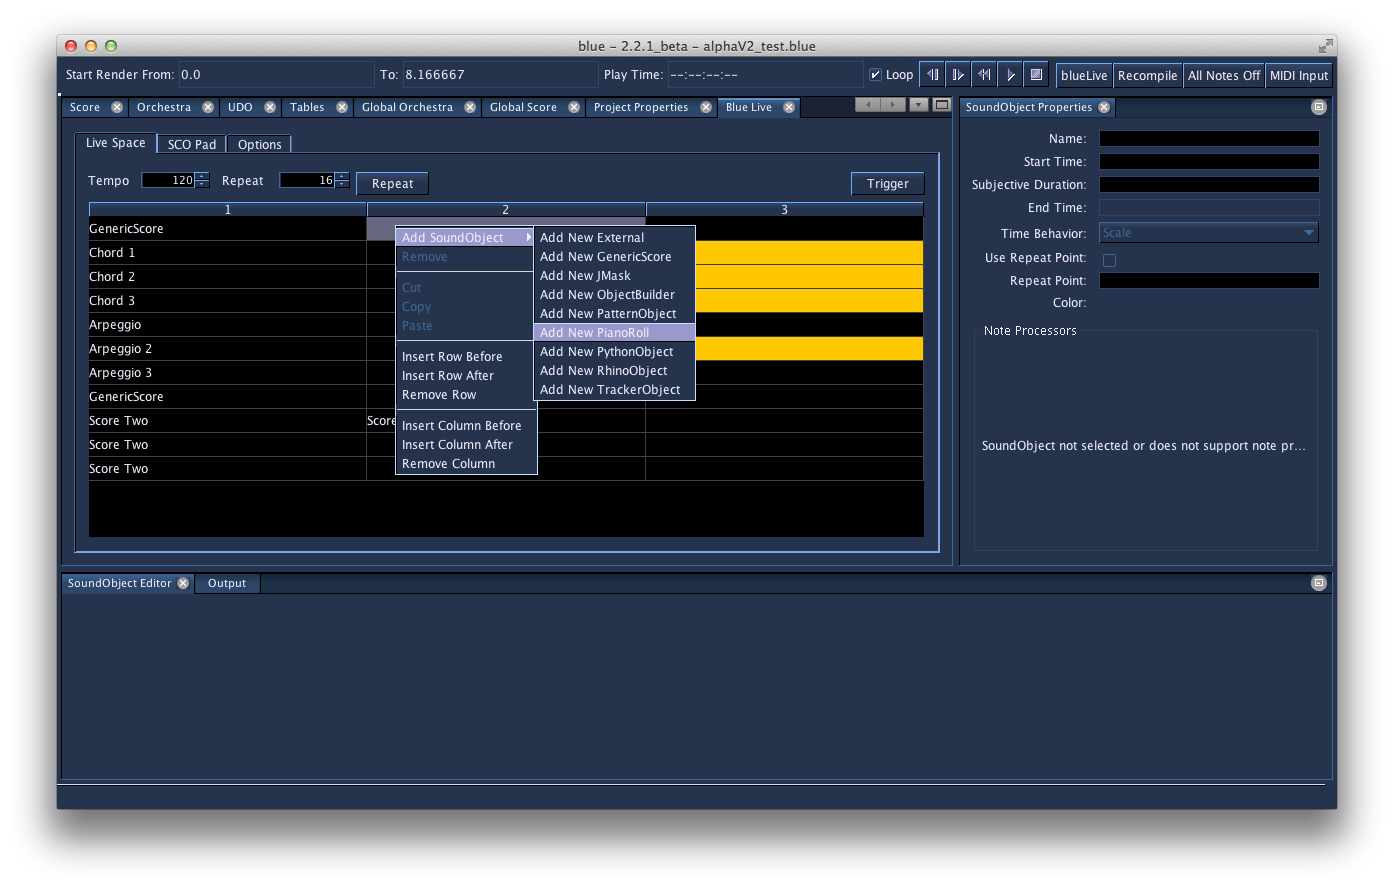
\includegraphics[width=1.00000\textwidth]{images/blueLive.png}

Blue Live allows you to work with Csound in realtime. It allows for
generating score with SoundObjects and working with MIDI keyboard input
to create notes and run with Csound instruments defined in your project.
Note: Blue Live works when using the Csound API, or on non-Windows
platforms when not using the Csound API. Windows does not allow piping
text to executable in a non-blocking way and therefore limits what can
be done when not using the API.

\subsection{Motivation}

The motivation of Blue Live is primarily to aid the composer in working
out ideas and to help configure instrument, effects, and mixer settings.
You may find it helpful early on within the life a composition, when you
want to try out a number of different ideas in realtime. You may tweak
instrument parameters, mixer settings, try out different notes and
chords with a MIDI keyboard, and even work with different SoundObjects.
Later, when you have some ideas worked out, you can take your
SoundObjects from blueLive into your score timeline and continue working
from there.

Beyond this primary capacity as a mode to aid composition, Blue Live has
some capacity to be used for realtime performance. The focus of Blue
Live's development is as a compositional aid first, and performance
second, though work continues to expand its usefulness in both regards.

\subsection{Working with Blue Live}

Blue Live is designed to work with the rest of your blue project file.
When Blue Live is turned on, the blue project generates everything from
the project except for the Score generated from the Score timeline. The
Global Score text will be used, but instead of
\textless{}TOTAL\_DUR\textgreater{} being calculated from the score
timeline, a default value of 3600 is used. This allows your notes that
would be used for effects instruments to run for 3600 seconds (this size
can be modified; please make a request if desired).

The main toolbar has four buttons for blue Live:

\begin{description}
\item[blueLive]
Toggle button that stops and starts blueLive
\item[Recompile]
If blueLive is running, this button will cause blue to recompile the CSD
from your project and restart blueLive. This is useful if you modify
your orchestra code and want to quickly recompile and continue working
with blueLive.
\item[All Notes Off]
Turns off any score notes that are actively playing
\item[MIDI Input]
Toggle button that turns on and off the configured MIDI devices setup in
Program Options (discussed further below).
\end{description}

The primary Blue Live window is available from the Window Menu, or by
using the ctrl-8 shortcut. The Blue Live window has three main tabs: the
Live Space, the SCO Pad, and Options. These will be discussed int he
following sections.

\subsection{Live Space}

The Live Space is an area to work with SoundObjects. It is a table
divided into bins and rows of spaces to place SoundObjects. SoundObjects
can be copied to/from the Score Timeline as well as the Live Space.
SoundObjects can also be created within the Live Space by right clicking
an empty bin within the bins and choosing "Add SoundObject" from the
popup menu. Clicking on an occupied bin will select that SoundObject.
The properties for the SoundObject can be modified using the SoundObject
Properties Window, and the contents of the SoundObject can be modified
from the SoundObject Editor Window. Besides the selected and unselected
states, you can double-click a soundObject to put it into an enabled
state. Enabled objects are highlighted in orange and are the
SoundObjects that are triggered when multi-trigger or repeat is used.

Once a SoundObject is added to the Live Space, it can be triggered in
one of two ways:

\begin{description}
\item[Single Trigger]
Trigger the contents of the currently selected SoundObject. This is done
by using the keyboard shortcut ctrl-T (cmd-T on OSX).
\item[Multi Trigger]
Triggers the contents of the currently enabled SoundObjects. This is
done either by using the Trigger button, or using the keyboard shortcut
ctrl-shift-T (cmd-shift-T on OSX).
\end{description}

Triggering a soundObject will take the score generated from it and pass
it immediately to the active Csound instance for blueLive (blueLive must
be running for this to work). Scores are always generated with Time
Behavior of None, processed through their NoteProcessors, then scaled
according to the given tempo.

One can turn on Repeat to cause repeated trigger of enabled SoundObjects
according to the tempo given and the number of beats in which to
retrigger. For example, using a repeat of 4 means it will re-trigger
every four beats. The score is processed as mentioned above, but there
is no truncation done. Therefore, if a SoundObject generates a score of
8 beats, and there is a repeat of 4 beats, when the repeat occurs, there
will be 4 beats of overlap between the first trigger and the second
trigger.

When Repeat is on, it will always finish out the current number of beats
in the repeat at the current tempo, before applying any changes to tempo
and repeat. Modifyications to tempo and repeat will apply then on the
next repeat trigger.

\subsection{SCO Pad}

\begin{quote}
\textbf{Note}

This feature will likely be removed in a future release.
\end{quote}

This is an experimental feature to record MIDI input in a manner similar
to to notation programs (press keys, then press 4 for a quarter note, 8
for and 8th note, etc.). This feature requires MIDI Input to be turned
on. This feature is experimental at this time.

\subsection{Options}

The options panel allows setting up parameters for blue Live. Currently
it contains options for modifying the commandline string used when
running blueLive. For most users, these modification will not be
necessary and the default commandline used will be sufficient.

\subsection{Working with MIDI}

blue's MIDI system, when enabled, will listen to configured MIDI devices
for notes, map the key and velocity, and generate Csound notes to
achieve MIDI-like note-on and note-off type behavior. This allows
working with a MIDI keyboard in realtime with your project instruments
without modifying your instruments specifically for MIDI. This also
means that when blue's MIDI system is enabled, Csound MIDI processing
should be disabled for your project.

To configure what MIDI devices to use, go to the program Options
settings (on OSX it is the application's Preferences, on other platofrms
it is the Options menu item in the Tools menu) and under "blue", go to
MIDI. There you will see a list of MIDI devices connected to your
computer. If you connected a device after starting blue, you can rescan
to find your MIDI device. In this window you will configure what MIDI
devices you want to use with blue, but these devices will not be opened
for listening until you enable MIDI Input on the blueLive toolbar in the
main application.

Once you have configured what devices to use with blue, return to the
main program and enable MIDI input using the "MIDI Input" button, then
start blueLive. At this point, when MIDI notes are played, blue will
take the incoming note data, map it according to the values configured
in the MIDI Input Panel window (available from the Windows Menu), and
then generate notes and pass them to Csound.

For a MIDI note on, blue will the channel number of the note and map it
to the instrument in the orchestra manager by index. For example, if you
have three instruments numbered 1, 3, and 5, notes for MIDI channel 1
will generate with instr 1, notes for MIDI channel 2 will generate with
instr 3, and notes for MIDI channel 3 will generate with instr 5.

The MIDI key number as well as the velocity will be mapped according to
the settings set in the MIDI Input Panel window. This allows for
generating frequency, Csound PCH, and using Scala Tuning files to
generate either frequencies or bluePCH format text, amongst other
values.

Instruments that are intended to be used with blue's MIDI system will
have to work with a 5 p-field note format. This does not mean your
instrument can only work with 5 p-fields, but rather that your
instrument must support at least that. An example blue project can be
found in examples/features/blueLiveMidi.blue (if you are using the OSX
application, you may need to explore the contents of the blue.app
program to find the examples folder).

\subsection{Exploring Ideas}

Blue Live uses a subset of the same soundObjects that are available on
the score timeline within the main editing window of blue. Some possible
ways you could explore ideas are:

\begin{itemize}
\item
  trying out SCO ideas with genericScore
\item
  testing your python functions with the pythonObject
\item
  testing your javaScript functions with the rhinoObject
\item
  using Cmask, nGen, Common Music, and other programs with the external
  soundObject to try out things live
\end{itemize}
